\chapter{Précision et rapidité des systèmes asservis\label{chap-perf}}

\minitoc
\newpage

\section{Introduction}

\section{Définitions de la précision}

Un système est précis si l'écart que l'on note $\epsilon(t)$ 
entre l'entrée $e(t)$ et la sortie $s(t)$ est nul.
Dans le domaine de Laplace, cet écart devient :
$$
\epsilon(p)=E(p)-S(p)
$$

On distingue deux cas :
\begin{itemize}
    \item En régime permanent, cet écart $\epsilon_s$ est nommée \textbf{erreur statique. }
    \item En régime transitoire, cet écart $\epsilon(t)=e(t)-s(t)$ est nommée \textbf{erreur dynamique.}
\end{itemize}

L'erreur dynamique consiste à suivre l'écart défini précedemment durant le transitoire.

Pour étudier l'erreur statique, on sollicite le système à différents types de signaux 
pour obtenir dans les différents cas :
\begin{itemize}
	\item l'\textbf{erreur indicielle} ou l'erreur de position qui est l'erreur statique de la réponse indicielle.
	\item l'\textbf{erreur de poursuite} ou erreur de vitesse qui est l'erreur statique de la réponse à une rampe.
	\item l'\textbf{erreur en accélération} qui est l'erreur statique de la réponse à une parabole.
\end{itemize}
Concrétement pour étudier l'erreur statique on cherche la limite à l'infini de $\epsilon(t)$
ou encore en appliquant le théorème de la valeur finale :
\begin{bequation}[ams align]
\epsilon(\infty)=\lim\limits_{t\to\infty} e(t)-s(t)=\lim\limits_{p\to 0} p\big(E(p)-S(p)\big)
\end{bequation}
Rappelons que pour pouvoir appliquer ce théorème la valeur finale doit être finie ou en d'autre
mot le système doit être stable.

\subsection{Précision en boucle ouverte}

Soit un système caractérisé par la fonction de transfert $H(p)$ 
est sollicité par l'entrée $E(p)$. La sortie $S(p)$ est alors donnée par :

\begin{center}
\tikzsetnextfilename{sb_bloc1-chap6_ext}
\begin{tikzpicture}
    \sbEntree{E}
	\sbBloc[3]{H}{$H(p)$}{E}
    \sbRelier[$E(p)$]{E}{H}
    \sbSortie[3]{S}{H}
    \sbRelier[$S(p)$]{H}{S}
\end{tikzpicture}
\end{center}

L'erreur statique est alors donnée par :
$$
\epsilon(\infty)=\lim\limits_{p\to 0} p\big(E(p)-H(p)E(p)\big)=\lim\limits_{p\to 0} p\big(1-H(p)\big)E(p)
$$

\subsubsection{Exemple d'un premier ordre}

%Rappelons qu'il est possible de corriger la précision 
%d'un système en boucle ouverte. 
Prenons l'exemple d'un système du 1er ordre de fonction de transfert canonique 
$H(p)=\dfrac{K}{1+\tau p}$ que l'on sollicite avec un échelon d'amplitude (consigne) 
$E_0$.
L'erreur statique est alors donnée par :
$$
\epsilon(\infty)=\lim\limits_{p\to 0} \left(1-\dfrac{K}{1+\tau p}\right)E_0=(1-K)E_0
$$

Le système est prècis (c.a.d $\epsilon(\infty)=0$) si $K=1$. 

%Il alors possible de corriger en boucle ouverte la précision en introduisant un gain $K'$ :

%\begin{center}
%\tikzsetnextfilename{sb_bloc2-chap6_ext}
%\begin{tikzpicture}
%    \sbEntree{E}
%	\sbBloc[3]{C}{$K'$}{E}
%    \sbRelier[$E(p)$]{E}{C}
%	\sbBloc[3]{H}{$\dfrac{K}{1+\tau p}$}{C}
%    \sbRelier[$U(p)$]{C}{H}
%    \sbSortie[3]{S}{H}
%    \sbRelier[$S(p)$]{H}{S}
%\end{tikzpicture}
%\end{center}
%tel que $K'K=1$ ou encore $K'=\frac{1}{K}$.

%Cependant, nous allons dans ce chapitre nous interesser uniquement à l'asservissement en 
%boucle fermée.

\subsection{Précision en boucle fermée}
Considérons le cas d'un système asservi de fonction de transfert $H(p)$
par une boucle de contre-réaction à retour unitaire.

\begin{center}
\tikzsetnextfilename{sb_bloc3-chap6_ext}
\begin{tikzpicture}
    \sbEntree{E}
	\sbComp{comp1}{E}
	\sbRelier[$E(p)$]{E}{comp1}
	\sbBloc[3]{H}{$H(p)$}{comp1}
    \sbRelier[$\epsilon(p)$]{comp1}{H}
    \sbSortie[3]{S}{H}
    \sbRelier[$S(p)$]{H}{S}
	\sbRenvoi[4]{H-S}{comp1}{}
\end{tikzpicture}
\end{center}

La~\gls{ftbo} est simplement donnée par $H(p)$. Dans le cas le plus
générale, il est toujours possible d'écrire une fonction de transfert
sous la forme canonique (\Cref{chap-slci}) :
$$
H_{BO}(p)=\dfrac{K}{p^\alpha}\cdot\dfrac{N(p)}{D(p)}
$$
avec $\alpha$ la classe du système en boucle ouverte, $K$ le gain statique et 
$N(p)$ et $D(p)$ de polynômes tels que $N(0)=D(0)=1$. 


Dans le domaine de Laplace l'écart $\epsilon(p)$ s'écrit :
$$
\epsilon(p)=E(p)-S(p)=\left(1-\dfrac{H_{BO}(p)}{1+H_{BO}(p)}\right)E(p)
$$
en remplaçant $H_{BO}(p)$ par sa représentation générale:
\begin{bequation}[ams align]
\epsilon(p)=\dfrac{p^\alpha D(p)}{p^\alpha D(p)+KN(p)}E(p)
\end{bequation}

L'erreur statique $\epsilon_s$


%\newpage
%%%%%%%%%%%%%%%%%%%%%%%%%%%%%%%%%%%%%%%%%%%%%%%%%%%%%%%%%%%%%%%%%%%%%%
%%%%%%%%%%%%%%%%%%%%%%%%%%%%%%%%%%%%%%%%%%%%%%%%%%%%%%%%%%%%%%%%%%%%%%
%%%%%%%%%%%%%%%%%%%%%%%%%%%%%%%%%%%%%%%%%%%%%%%%%%%%%%%%%%%%%%%%%%%%%%
%\section*{Exercices du chapitre}
%%%%%%%%%%%%%%%%%%%%%%%%%%%%%%%%%%%%%%%%%%%%%%%%%%%%%%%%%%%%%%%%%%%%%%
%%%%%%%%%%%%%%%%%%%%%%%%%%%%%%%%%%%%%%%%%%%%%%%%%%%%%%%%%%%%%%%%%%%%%%
%%%%%%%%%%%%%%%%%%%%%%%%%%%%%%%%%%%%%%%%%%%%%%%%%%%%%%%%%%%%%%%%%%%%%%


%\exercice{}
%\question

%\newpage
%%%%%%%%%%%%%%%%%%%%%%%%%%%%%%%%%%%%%%%%%%%%%%%%%%%%%%%%%%%%%%%%%%%%%%
%%%%%%%%%%%%%%%%%%%%%%%%%%%%%%%%%%%%%%%%%%%%%%%%%%%%%%%%%%%%%%%%%%%%%%
%%%%%%%%%%%%%%%%%%%%%%%%%%%%%%%%%%%%%%%%%%%%%%%%%%%%%%%%%%%%%%%%%%%%%%
%\section*{Corrigé des exercices}
%%%%%%%%%%%%%%%%%%%%%%%%%%%%%%%%%%%%%%%%%%%%%%%%%%%%%%%%%%%%%%%%%%%%%%
%%%%%%%%%%%%%%%%%%%%%%%%%%%%%%%%%%%%%%%%%%%%%%%%%%%%%%%%%%%%%%%%%%%%%%
%%%%%%%%%%%%%%%%%%%%%%%%%%%%%%%%%%%%%%%%%%%%%%%%%%%%%%%%%%%%%%%%%%%%%%


